\documentclass[a4paper]{article}
\usepackage[utf8]{inputenc}
\usepackage{underscore}
\usepackage[english,serbian]{babel}
\usepackage{graphicx}
\usepackage{color}
\usepackage{url}
\usepackage{float}

\usepackage[unicode]{hyperref}
\hypersetup{colorlinks, citecolor=green, filecolor=green, linkcolor=blue, urlcolor=blue}

\begin{document}

\title{Nanotehnologija i primene\vspace{0ex}\\
\small{Seminarski rad u okviru kursa\\
Tehničko i naučno pisanje\\
Matematički fakultet}\vspace{3ex}}
\author{
Petar Đerić\\
mi20135@alas.matf.bg.ac.rs\\\\
Ivan Tešović\\
mi20111@alas.matf.bg.ac.rs\and
Luka Mijailović\\
mi22100@alas.matf.bg.ac.rs\\\\
Uroš Cvetković\\
mi22065@alas.matf.bg.ac.rs
}
\date{Novembar 2022.}

\maketitle

\abstract{U narednom tekstu ćemo se ukratko upoznati sa pojmom \textbf{nanotehnologije.} Na početku ćemo govoriti o istoriji (razvoju nanotehnologije), nakon čega će biti reči o njeim primenama u raznim interesantnim oblastima, kao i o \textbf{nanomaterijalima}.}
 
\tableofcontents                 
\newpage

\section{Uvod}
\label{sec:uvod}
\sloppy \textbf{Nano} predstavlja milijarditi deo metra i bez mikroskopa uopšte nije vidljiv. Materijali se u sitnijoj razmeri ponašaju sasvim drugačije nego u većem obliku. Da bi se omogućilo poboljšanje performansi i osobina materijala, \textbf{nano čestice} su u sve većem fokusu istraživanja.\\ Osnovni cilj izučavanja na ovom nivou jeste sposobnost razumevanja materijala na \textbf{nano-lestvici}. Ove mikro veličine su bitne kada se proučava susret dva materijala.\\ Kod dimenzija u opsegu do 100 nm, pojave kvantne fizike preovladavaju nad pojavama klasične fizike. Bitna je činjenica da manja tela imaju znatno veći odnos broja atoma na površini i broja atoma u unutrašnjosti od većih tela.\\ Ti odnosi na mikro nivou dovode do razumevanja kompletne strukture materijala, a mogućnost upravljanja složenim strukturama se vrši upravo u nano području. Nevidljiva revolucija ima tendenciju da preraste u novu industrijsku revoluciju.


\section{Nanotehnologija}

\subsection{Nastanak i razvoj nanotehnologije}
\sloppy Iako se nanotehnologija smatra modernom naukom, njeni počeci se vezuju za duboku prošlost.
Termin "\textbf{nanotehnologija}“, prvi je upotrebio \textbf{Norio Taniguči} (Slika \ref{slika_Norio}) sa Univeziteta u Tokiju 1974. godine govoreći o proizvodnji materijala u slučaju kada je tolerancija na grešku reda \textbf{nanometra}.
Krajem 1980-ih, pojam nanotehnologija ulazi u široku upotrebu za opis budućih tehnologija koje će se bazirati na molekularnim mašinskim sistemima koji su dizajnirani tako da budu sposobni za konstruisanje složenih proizvoda sa atomskom preciznošću.\\ 
Od sredine 1990-ih, upotreba koncepta se proširila na instrumente, procese i proizvode čije su ključne dimenzije u rangu između 1 i 100 nanometara.\\

\begin{figure}[H]
    \centering
    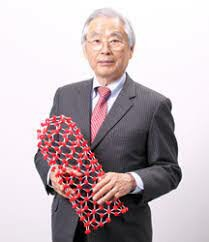
\includegraphics[width=.4\textwidth]{slika 1.jpg}
    \caption{Norio Taniguči}
    \label{slika_Norio}
\end{figure}

\subsection{Pojam nanotehnologije}
\textbf{Nanotehnologija} je interdisciplinarna nauka koja uključuje fiziku, hemiju, biologiju, nauke o materijalima, kao i širok skup inženjerskih disciplina.\\ 
Danas, nanotehnologija kao inženjerska disciplina, odnosi se na tehnike i proizvode koji uključuju strukture nanometarskih dimenzija ( od 1 do 100 nanometara).\\  Reč \textit{nanotehnologija}, koristi se kao sinonim i za \textbf{nauku} i za \textbf{tehnologiju}.\\ 
Kao nauka, nanotehnologija proučava fizičke, hemijske i biološke osobine molekula i atomskih čestica. Kao tehnologija, primenjuje istraživanja iz navedenih nauka i različite inženjerske discipline za proizvodnju materijala i funkcionalnih sistema sa posebnim osobinama.

\subsection{Ciljevi i mogućnosti nanotehnologije}
Progres u nanotehnologiji se može posmatrati preko mnogih parametara, uključujući preciznost, složenost, isplativost i izbor proizvoda.\\ 
Dugoročni ciljevi nanotehnologije su atomska preciznost, ušteda u proizvodnji, kao i masovna proizvodnja. Kombinacija ovih ciljeva deluje izvodljivo, ali samo kroz višeslojni proces koji počinje sa razumjevanjem da je trenutno stanje razvoja nanotehnologije ograničenih sposobnosti.

Tehnologije koje se koriste u nanotehnologiji su veoma različite, brzo se menjaju i često nisu međusobno povezane. Tipični proizvodi nanotehnologije su \textbf{nanočestice}, \textbf{fibre} i \textbf{filmovi} različitih materijala i struktura. 
Mediji i materijali koji se koriste za proizvodnju nanostruktura i nanotekstura nalaze praktičnu primjenu počev od proizvodnje odeće otporne na fleke, pa sve do naprednih elektronskih komponenti.

Sa razvojem nanotehnologije, razviće se nove metode lečenja koje su bazirane na upotrebi nano-robota, popularno nazvanih nanobotovi (eng. nanobots). Već su razvijeni materijali koji se mogu samopopravljati (eng. self-healing materials) i to je verovatno pravac kojim će se oblast proizvodnje novih materijala kretati.\\
Budućnost bi trebalo da donese razvoj aktivnih nanostruktura, zatim konkretnih funkcionalnih nanosistema, i konačno polovinom ovog veka i do razvoja savršenih molekularnih nanosistema.
\end{document}
